\section{Company information}

\subsection{Organization}
When we talk about company information, we focus our interest on the points
that can give us a detailed view of the entire business and its processes. This
type of essential information is usually found on the target company's
websites. We will not necessarily find all the necessary information to give us
an {\bf insight} into the company and its {\bf processes}. This could tell us which
companies will be most interested in working with our target company and which
requirements must be met. Understanding our target company's business processes
can give us an idea of how to structure our attacks. Therefore we can design
our attacks to be executed during a specific step in the process.

We can also get an insight into the company's dependencies. From this, we will
be able to conclude which technologies are needed to manage the company, which
will indicate how the company may be structured from an infrastructure
perspective.
\begin{figure}
  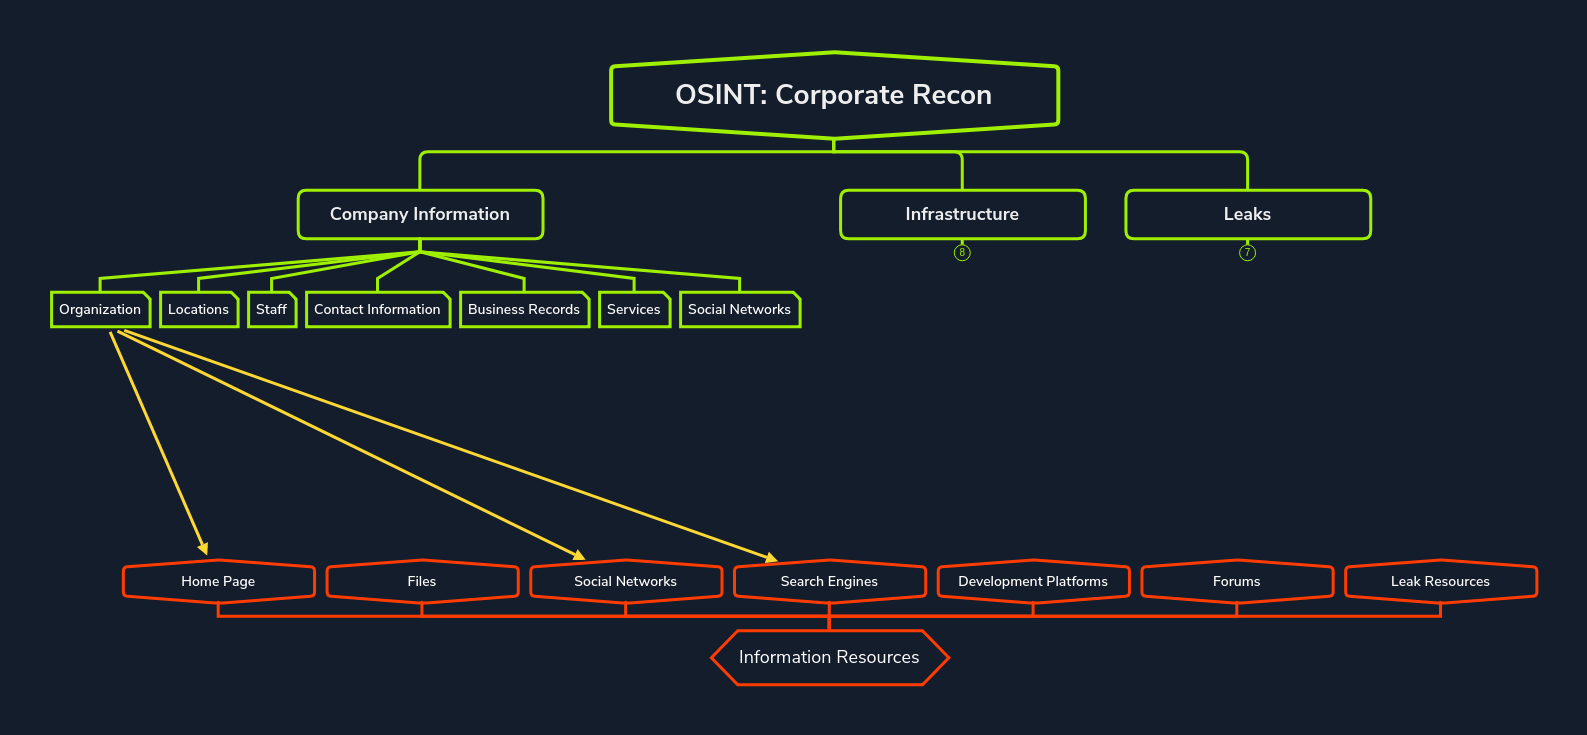
\includegraphics[width=\linewidth]{recon/osint/images/osint-org.png}
  \caption{OSINT Organization}
  \label{fig:osint-org}
\end{figure}

Generally, the company's home page, social networks, and search engines can be
used to map out the company's organizational structure. There are no useful
tools that can be used to map out the company's organizational structure
efficiently. Instead, we must rely on the logical association between the
information we will find during OSINT and the actual intelligence.

Furthermore, it is challenging to keep it dynamic because every company has
unique staffing needs and employees, all of whom bring different strengths,
weaknesses, and abilities. Therefore this field of OSINT is more a repeatable
process than a static method.

\subsubsection{Locations}
If our engagement is a red team assessment, then such information is much more
relevant than a regular penetration test procedure. Red-teaming can also
include, among other things, the physical security of the company and is used
to determine which methods and techniques can be used to obtain highly
sensitive information that may not be accessible from the internet. The
company's locations are of great importance for this. However, the scope and
rules for which procedures may and may not be used must be strictly observed.

Companies already pay a lot of money to attract potential customers by
presenting themselves to their customers in the best possible way and sell
themselves better from a marketing point of view. Here we can always ask
ourselves when the company would arouse our {\bf interest}.

\begin{figure}
  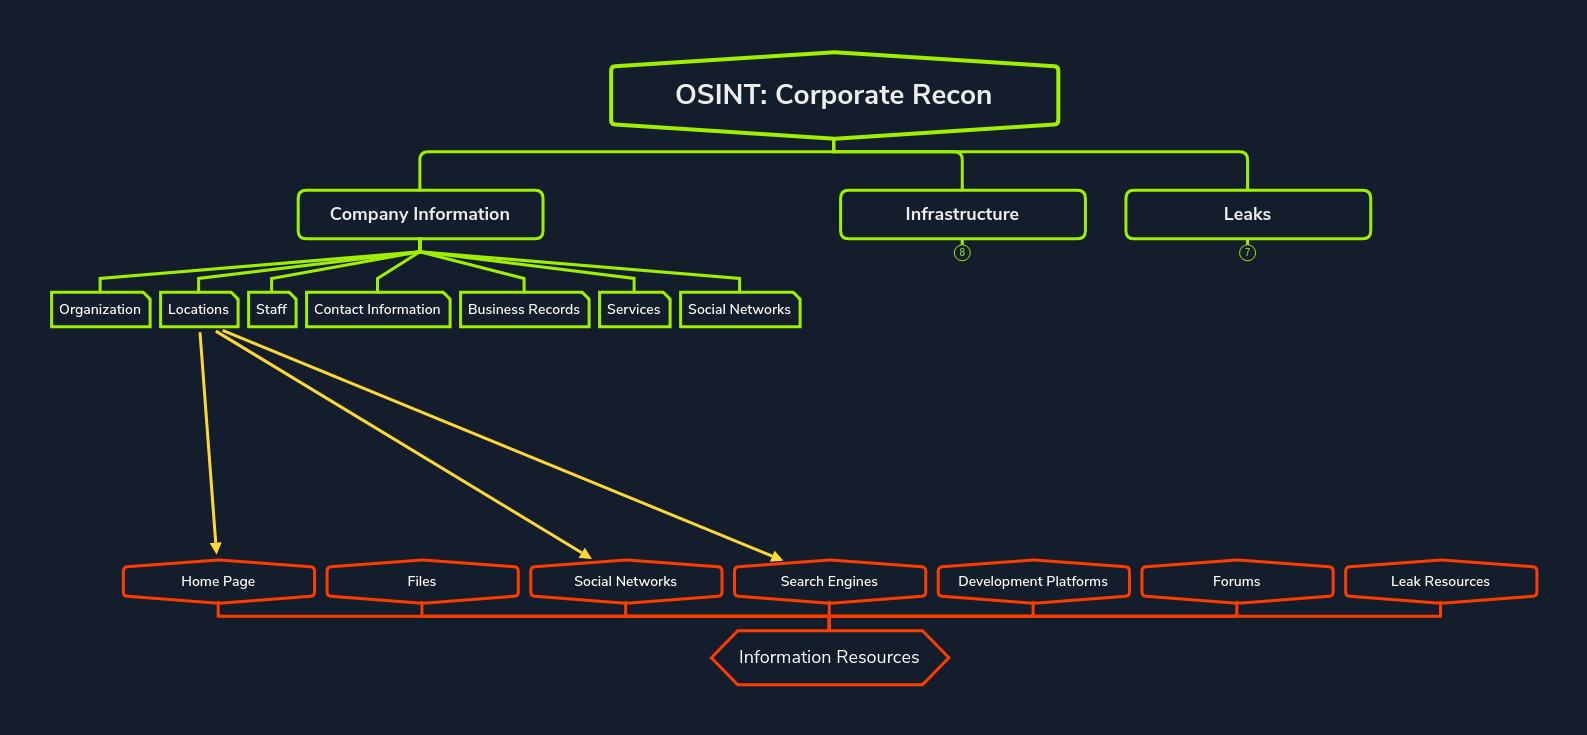
\includegraphics[width=\linewidth]{recon/osint/images/osint-locations.png}
  \caption{OSINT Locations}
  \label{fig:osint-locations}
\end{figure}

\subsubsection{Staff}
Every company's marketing department attaches great importance to the best
possible representation of its {\bf staff} so that potential customers can be
sure they will be taken care of in a professional manner. The company's
employees handle all the processes. We are interested in the information they
use to interact with the company and its infrastructure. This may include but
is not limited to email addresses, phone numbers, usernames, passwords, and the
social networks on which they operate.

The employee's role in the company can also be used to assess their privileges
in specific areas. Thus, a manager would likely have higher rights than
customer support. However, even if a secretary does not have direct access to
the systems, the individuals in these roles can be an attractive attack vector
for us since they most likely have full access to calendars, plans, contact
data, email addresses, and more.

\begin{figure}
  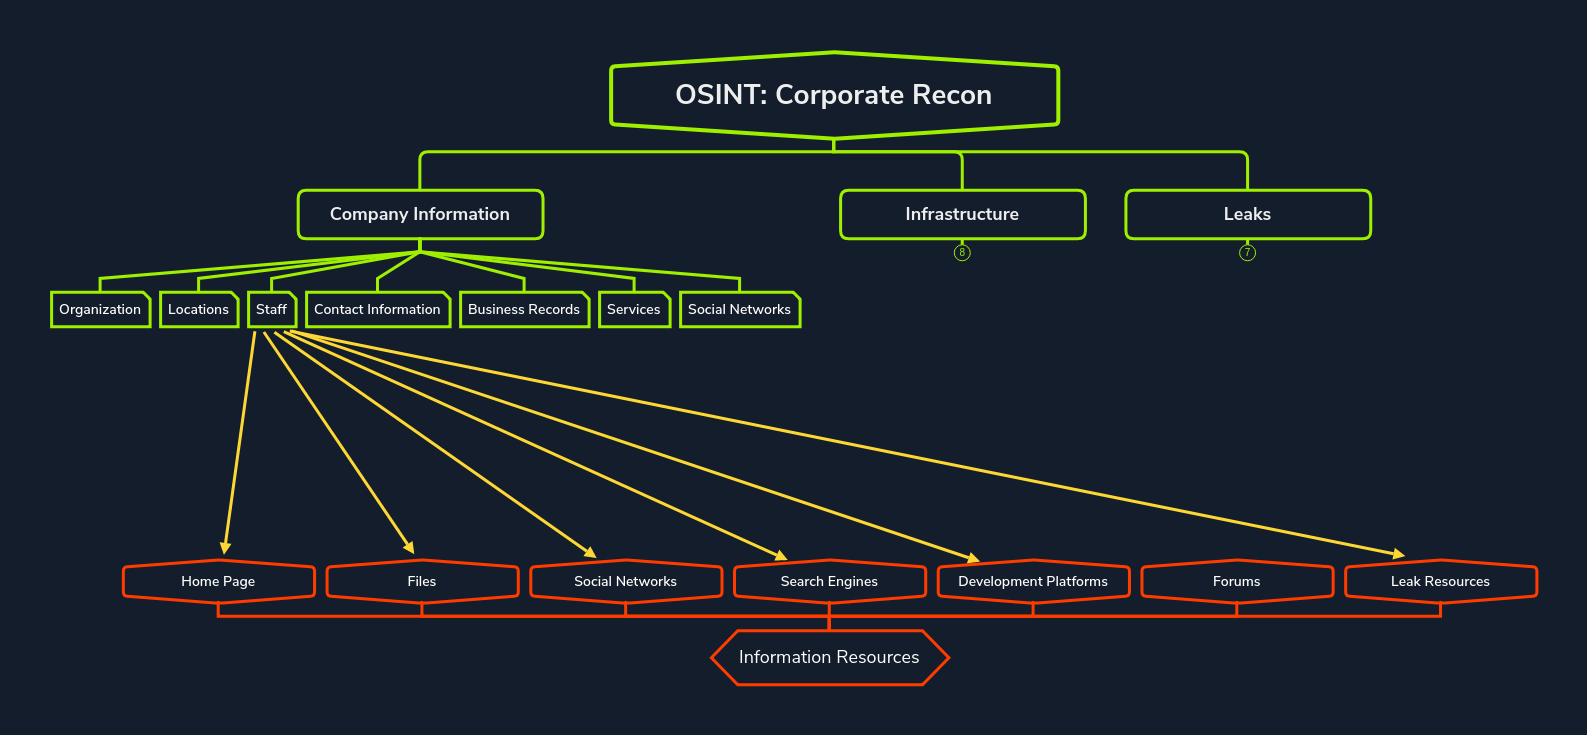
\includegraphics[width=\linewidth]{recon/osint/images/osint-staff.png}
  \caption{OSINT Staff}
  \label{fig:osint-staff}
\end{figure}

\subsubsection{Contact Information}
Another critical point for all potential customers is the company's
accessibility. For this reason, {\bf contact details} are always disclosed.
After all, customers may want to find out more about the company or even
arrange a meeting. Contact information includes phone numbers and email
addresses, and usernames from various communication portals such as Skype,
Microsoft Teams, Slack, Discord, etc. These usernames can also be associated
with the employees. This part of OSINT will be discussed in more detail at {\bf
OSINT: Staff Investigation}.

\begin{figure}
  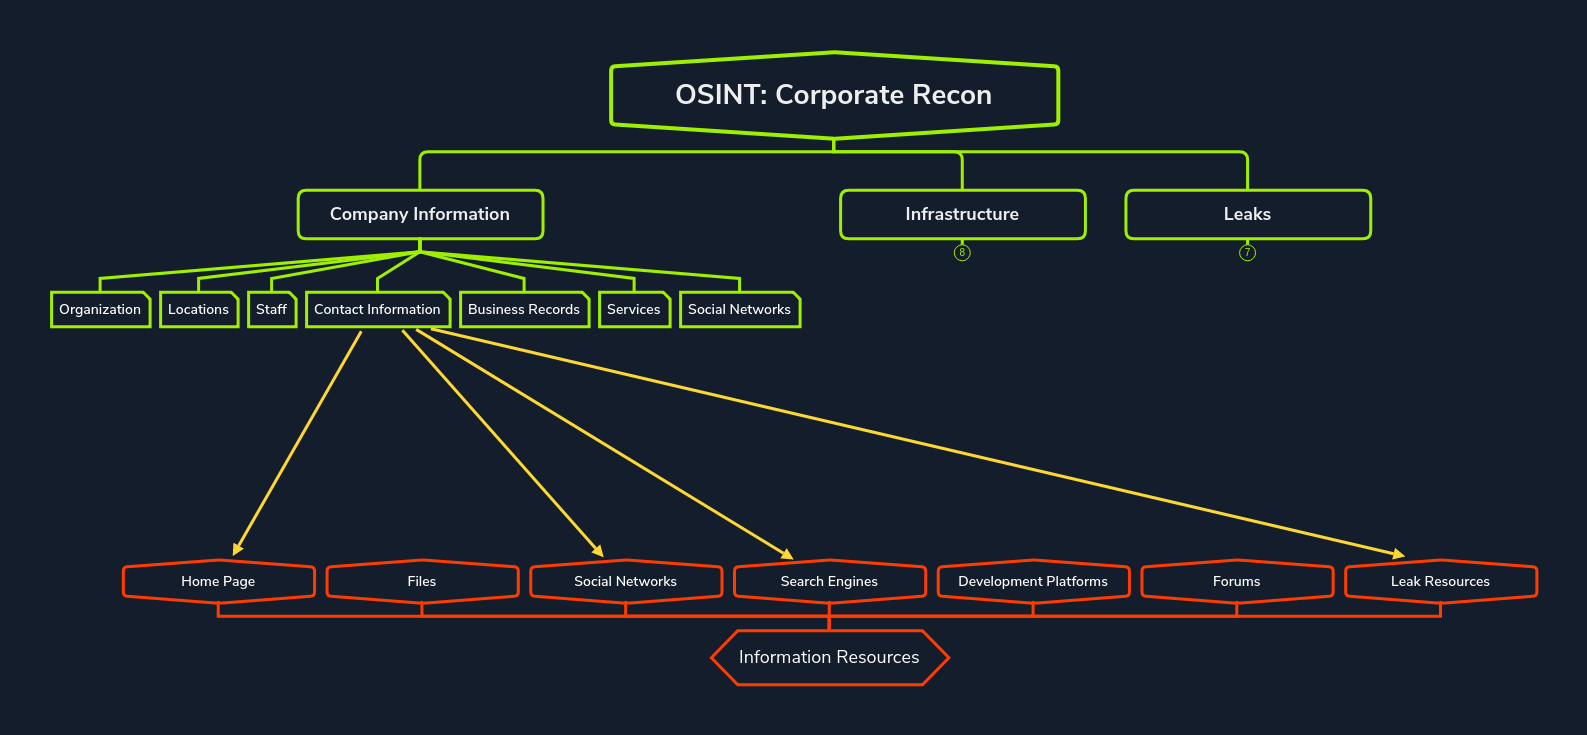
\includegraphics[width=\linewidth]{recon/osint/images/osint-contact.png}
  \caption{OSINT Contact}
  \label{fig:osint-contact}
\end{figure}

\subsubsection{Business records}
Significant customers look at the company's website and the {\bf business
records}, to learn more about it. From an OSINT perspective, they can also tell
us a lot about its progress. These include the company's {\bf locations}, {\bf
financial situation}, {\bf references}, and {\bf reputation}. We are
particularly interested in poor feedback about the company.

Poor feedback requires poor communication and the resulting i{\bf failures in
the business processes}. If a customer's inquiry or request is not fulfilled,
it may not always be a human mistake on the part of the employee but may
indicate technical issues. Companies often try to "hide" this feedback not to
create a wrong impression for potential customers.

Business records also include the degree of recognition in the market. For
example, we can get this through reviews by (former) employees or on social
networks. Customer satisfaction also plays a role. We can conclude how
structured and coordinated the company works internally to complete its
services and overcome customer problems for the services provided.

The company's financial situation tells us a lot about its commitment and
productivity. If a company continually offers new products and services, it can
positively affect its financial situation. Depending on the company's size, the
downside of this is that it can lead to chaotic processes. This can mean a
great deal of organizational effort and communication. Therefore, it leads to a
higher risk of phishing attacks because the content of a detailed, customized
phishing email is rarely actually checked.

\begin{figure}
  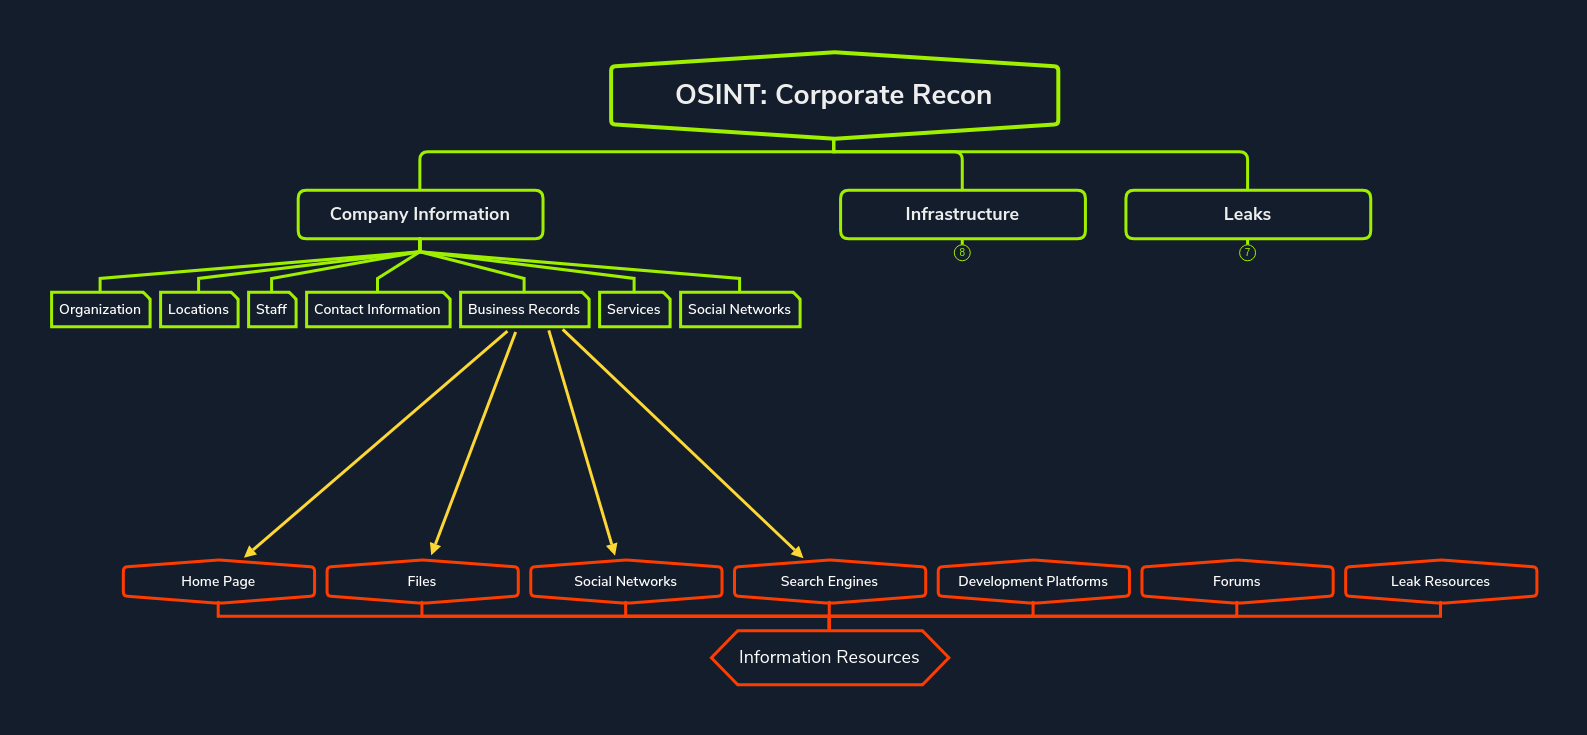
\includegraphics[width=\linewidth]{recon/osint/images/osint-business-records.png}
  \caption{OSINT Business records}
  \label{fig:osint-business-records}
\end{figure}

\subsubsection{Services}
{\bf Services} are also explained in great detail on the website so that the
number of external inquiries is kept to a minimum. For this reason, how each
service is carried out is usually discussed in detail. All other questions that
arise are generally specific.

\begin{figure}
  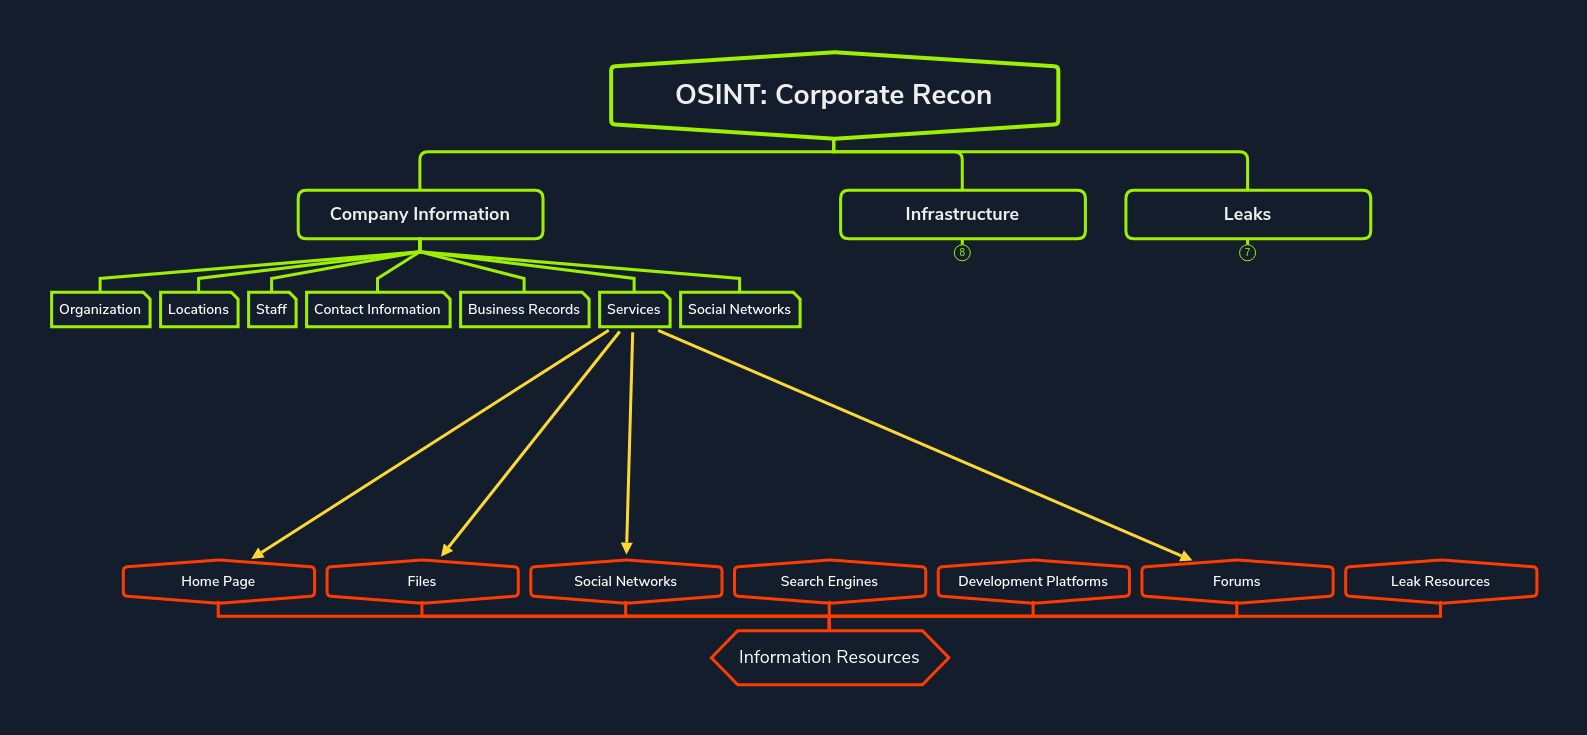
\includegraphics[width=\linewidth]{recon/osint/images/osint-services.png}
  \caption{OSINT Services}
  \label{fig:osint-services}
\end{figure}

\subsubsection{Social Networks}
We can also ask where to find more information about the company during a phone
call. We are usually directed to {\bf blog posts}, {\bf videos}, or {\bf
documentation} from a marketing perspective that would give us better insight
into the company. We can find a variety of information about the target company
through the different social media networks. We usually first direct our focus
to the company's linked accounts via its home page. In turn, these may lead us
to different sources of information not mentioned on the home page.

We can also search the different platforms themselves to see where the company
is represented on social networks. Finally, we can use search engines or forums
to find out if the company is mentioned there.

\begin{figure}
  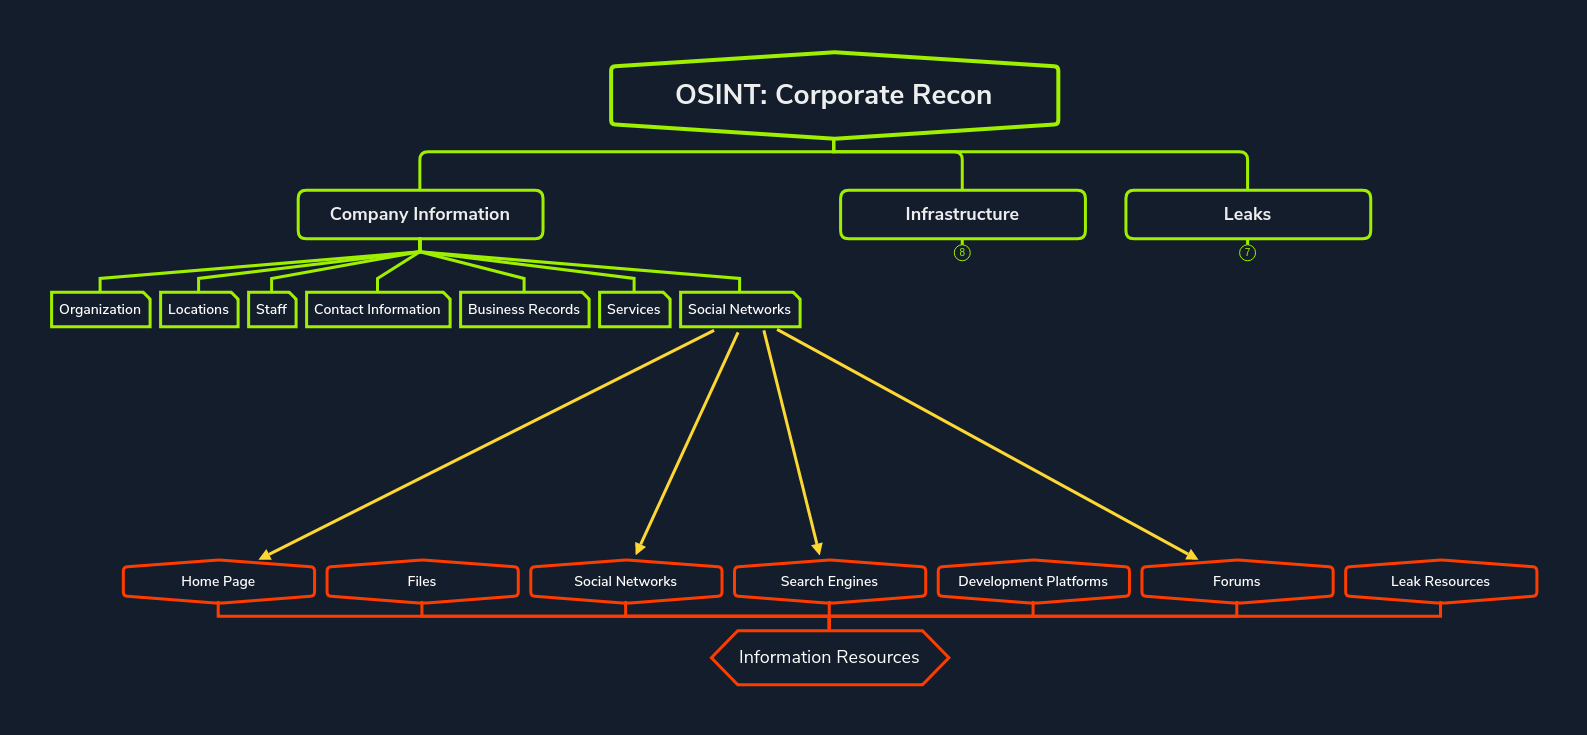
\includegraphics[width=\linewidth]{recon/osint/images/osint-social.png}
  \caption{OSINT Social}
  \label{fig:osint-social}
\end{figure}

\subsection{Locations}
When we look into a company's locations, we have to identify the most obvious
locations in advance. Larger companies that are active in the field of
production sometimes have sites that they do not mention. These can also be
identified in the OSINT process. The most prominent locations are usually
listed on the company's home page. After all, the company wants to attract
potential customers with the number of locations it has. It is an overall
strategy for companies to present themselves as the best all over the world.
This contributes significantly to marketing and increases the number of
customers and thus the turnover.

In general, we can find basic information about a company's locations in
advance using the following resources

\subsubsection{Home Page}
If we start with the home page and browse through the site a little, we will
find {\bf countries}, {\bf cities}, {\bf addresses}, and possibly even maps
that show the company's locations. 

Most of the time, we will also find lists that include the countries and/or
cities where the company has its offices. These locations are usually managed
locally by administrators but also may be managed centrally. If the company is
centrally managed, these locations (either the entire company or specific
locations) within the scope can also provide us with attack vectors that we can
use to get into the systems' central administration infrastructure.

\subsubsection{Social Networks}

Social networks are used to share much information, especially information that
potential customers can use to learn more about the company. This includes the
publication of locations of offices or production facilities. This type of
information can be found on many social networks such as Twitter, LinkedIn,
Instagram, Snapchat, YouTube, WeChat, Facebook, and others. Most links to a
company's social networks can be found on their home page.

\subsubsection{Search Engines}

Every company location can provide us with another potential attack vector,
whether physical or technical. Each site has different employees and managers
who have their way of working and can open up different attack paths for us
than other locations. As soon as we have detailed information about the
locations, we should document them and, in the best case, add a graphical
representation as evidence in our documentation. For example, we can use
\href{https://maps.google.com/}Google Maps},
\href{https://earth.google.com/web/}{Google Earth},
\href{https://showmystreet.com/}{ShowMyStreet}, and many others to obtain these
types of views.

In this case, we could pretend to be a significant client for potential
collaboration and organize a meeting to be let into the building and get a much
better insight into the company's processes. If the contract requires a
physical test, we can also get an inside view of the building's physical
security, such as door locks, windows, security, cameras, rooms, departments,
and more.

Information about locations is mainly interesting for {\bf physical Red Team}
operations. This is because it distinguishes between the times at which a
"break-in" can be most efficient. If a physical assessment is conducted during
working hours, we must be granted appropriate access to restricted areas
upfront. If possible, it is better to find a way to enter the building at night
if the alarm systems and their vulnerabilities allow it. The locations
themselves are the company's buildings and the location of the offices.
Sometimes there are also badge readers that we can see and use to identify how
to set up our cloner to hijack access cards wirelessly.

Suppose a manager or even higher employee feels safe in their office, which has
only access to a minimal number of employees and suddenly finds a USB stick on
their desk. In that case, they may wonder where it came from. The feeling of
being safe increases the likelihood that the USB stick we leave behind will be
plugged into their computer.

In larger companies, we will find some of these locations, which at first
glance already indicate some potential weaknesses in the field of physical
security. Suppose we have such an assignment where we also have to test the
organization's physical security. In that case, we can use the same resources
to get a picture of the terrain or even physically walk through the location as
a "passerby" and record a video of the terrain with a simulated phone call.
Depending on whether the location and the terrain allow it, we can also take
photos from a distance. By using the online resources, we will also be able to
gain some information.

We have to keep in mind that these photos have not been made today and may not
be up to date. Nevertheless, if we take a closer look at them, we can see some
interesting characteristics of the building, which could be helpful for us.

\subsection{Staff}


\subsection{Contact information}

\subsection{Business records}

\subsection{Services}

\subsection{Social Networks}
